%%%%%%%%
\documentclass [11pt, a4paper, leqno] {article}
\usepackage [polish] {babel}
\usepackage {polski}
\usepackage [utf8] {inputenc}
\usepackage [T1] {fontenc}
\usepackage {indentfirst}
\usepackage {setspace}
\usepackage {amstext}
\usepackage {amsfonts}
\usepackage {graphicx}
\DeclareGraphicsExtensions{.png}
\setstretch {1.15} %interlinia
\frenchspacing
\renewcommand {\thesection} {\arabic{section}.}
\renewcommand {\thesubsection} {\arabic{section}. \arabic{subsection}.}
\renewcommand {\thesubsubsection} {\arabic{section}. \arabic{subsection}. \arabic{subsubsection}.}
\textheight 610pt
\makeatletter
\renewcommand\@biblabel[1]{#1}
\makeatother
\usepackage[a4paper,left=3.8cm,right=3.8cm,top=3.3cm,bottom=3cm]{geometry}
%%%%%%%%

\begin{document}
% STRONA TYTUŁOWA

\begin{center}
  \thispagestyle{empty} %usunięcie numeracji
  {\large Studencka Pracownia Inżynierii Oprogramowania} \\ [0.5cm]
	{\large Instytut Informatyki Uniwersytetu Wrocławskiego} \\ [6.0cm]

  {\large Rafał Florczak, Dominik Rabij} \\ [1.5cm]

	{\huge Dokumentacja oprogramowania} \\ [0.5cm]
  {\huge RECEPCJONISTA} \\ [1.5cm]

  {\large Plan bazy danych} \\ [0.5cm]

  \vfill
  
  {\large Wrocław, \today} \\ [0.5cm]
  %{\large Wrocław, 6 listopada 2015} \\ [0.5cm]
  {\large Wersja 0.1}
\end{center}

\newpage

% TABELKA WERSJI

\textit{Tabela 0.} Historia zmian dokonanych w dokumencie

\begin{center}
  \begin{tabular}{| l | l | l | l |}
    \hline
    \multicolumn{1}{|c|}{Data} & 
    \multicolumn{1}{|c|}{Numer wersji} &  
    \multicolumn{1}{|c|}{Opis} &
    \multicolumn{1}{|c|}{Autor} \\ \hline \hline
    2015-12-16 & 0.1 & Utworzenie dokumentu & Rafał Florczak \\ \hline
  \end{tabular}
\end{center}

\medskip

\tableofcontents

\newpage

\section{Wprowadzenie}

\subsection{Cel dokumentu}
\noindent
Celem niniejszego dokumentu jest przedstawienie rozwiązań wybranych przez projektantów bazy danych. Opisany zostanie wybrany system zarządzania bazą danych oraz schemat relacji. Są one kluczowe dla sprawnego działania Recepcjonisty.

Dokument jest przeznaczony dla programistów oraz osób, które będą zajmowały się utrzymaniem oprogramowania w przyszłości.

\section{Baza danych}
\subsection{System zarządzania bazą danych}
\noindent
Do przechowywania i nadzoru nad zasobami bazy danych wybrany został system PostgreSQL, ponieważ jest on darmowy, stabilny, szybki, popularny, a jego kod jest dostępny publicznie.

\subsection{Schemat bazy danych}


\begin{center}
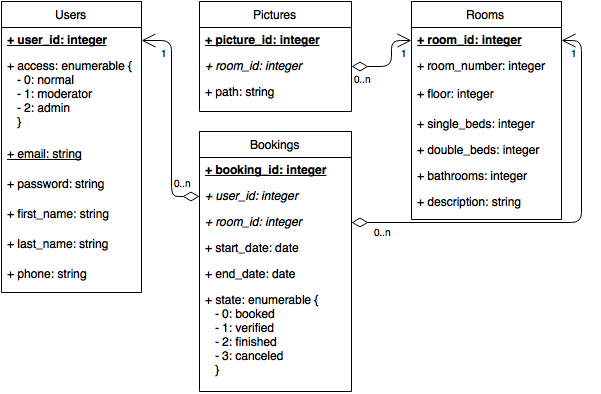
\includegraphics[scale=0.7]{recepcjonistadb}
\textit{Rysunek 1.} Schemat bazy danych
\end{center}

\newpage
\noindent
Opis notacji: 
\begin{itemize}
  \item podkreślenie --- klucz relacji,
  \item pogrubienie --- klucz główny relacji,
  \item pochylenie --- klucz obcy,
  \item $\Diamond$---------> --- relacja jeden-do-wielu.
\end{itemize}

\subsubsection{Użytkownicy (users)}
\noindent
Tabela przechowuje informacje o wszystkich użytkownikach Recepcjonisty --- zarówno o klientach, jak i  jego obsłudze. Polem wartym uwagi jest \textit{access}, które oznacza poziom dostępu danego użytkownika.

\subsubsection{Rezerwacje (bookings)}
\noindent
Relacja zawiera informacje o złożonych rezerwacjach (także tych zakończonych i anulowanych).

\subsubsection{Pokoje (rooms)}
\noindent
Tabela przedstawia dane o pokojach w hotelu. Informacja o liczbie łóżek została rozdzielona na dwa odrębne pola --- \textit{$single_{-}beds$} oraz \textit{$double_{-}beds$} oznaczające odpowiednio liczbę łóżek jednoosobowych i dwuosobowych.

\subsubsection{Zdjęcia (pictures)}
\noindent
Relacja przechowuje ścieżki do zdjęć poszczególnych pokojów.


\end{document}